\subsection{The geometry of one cut}

\begin{figure}[htbp]
\centering
\includegraphics[width=\textwidth]{flipped_vgmm_cut_z_0.39_error.png}
\caption{The cut at $z=0.39$, the one with the largest curvature
  mismatch of the four. Left: the meridian half plane. Branch~1 (blue) is
  the bowl. Branch~2 (red) is the cap, reflected down across the cut
  plane, so it runs \emph{inside} the bowl and the two meet at the star
  in a crease of $81.8^\circ$. The two arrows are the outward tangents
  the glue rotation is built from. Right: the surface $\Linf$ error
  against $h$. The heavy black line is the uncut solve with the crease
  ignored; it is flat. The three glued variants lie on top of one
  another, and their sawtooth is the grid-alignment scatter, not a
  failure of the solve.}
\label{fig:cut039}
\end{figure}

\subsection{The glue is what makes the solve converge}

The clearest result of this test is the gap between the baseline and the
glued solves. Table~\ref{tab:cut039} gives the cut at $z=0.39$ in full.

\begin{table}[htbp]
\centering
\caption{Surface $\Linf$ error of $u$, flipped ellipsoid, cut at
  $z=0.39$ ($\varphi_c = 0.9273$, $\kappa_m = 1.2986$,
  $\kappa_p = 0.8187$, glue angle $1.4282$~rad $= 81.8^\circ$,
  $\dk = 3.0703$). The rate under each error is the level-to-level
  ratio. Only the fitted slope is a rate; see
  Section~\ref{sec:scatter}.}
\label{tab:cut039}
\small
\begin{tabular}{@{}r rr rr rr rr@{}}
\toprule
 & \multicolumn{2}{c}{uncut, crease ignored}
 & \multicolumn{2}{c}{rotation from $d_k$}
 & \multicolumn{2}{c}{rotation from $d_{k2}$}
 & \multicolumn{2}{c}{exact $R$} \\
\cmidrule(lr){2-3}\cmidrule(lr){4-5}\cmidrule(lr){6-7}\cmidrule(lr){8-9}
$h$ & error & rate & error & rate & error & rate & error & rate \\
\midrule
0.0650  & 4.071e-01 & --    & 2.101e-02 & --    & 6.599e-02 & --    & 2.244e-02 & --    \\
0.0533  & 3.467e-01 & 0.81  & 1.149e-02 & 3.04  & 1.697e-02 & 6.84  & 1.145e-02 & 3.39  \\
0.0437  & 3.566e-01 & $-0.14$ & 3.057e-03 & 6.67  & 5.507e-03 & 5.67  & 3.261e-03 & 6.33  \\
0.0358  & 2.970e-01 & 0.92  & 1.074e-02 & $-6.33$ & 1.149e-02 & $-3.70$ & 1.089e-02 & $-6.07$ \\
0.0294  & 5.391e-01 & $-3.00$ & 3.403e-03 & 5.79  & 3.046e-03 & 6.69  & 3.356e-03 & 5.93  \\
0.0241  & 2.836e-01 & 3.24  & 6.445e-03 & $-3.22$ & 6.414e-03 & $-3.75$ & 6.436e-03 & $-3.28$ \\
\midrule
\multicolumn{1}{@{}l}{fitted}
        & \multicolumn{2}{c}{\textbf{0.10}}
        & \multicolumn{2}{c}{1.20}
        & \multicolumn{2}{c}{2.31}
        & \multicolumn{2}{c}{\textbf{1.26}} \\
\bottomrule
\end{tabular}
\end{table}

Three things are worth reading off it.

\paragraph{The baseline does not converge.} The uncut vGMM solve, which
applies the closest point method to the creased surface as if the crease
were not there, has a fitted slope of $0.10$. Its error stays between
$0.28$ and $0.54$ at every grid spacing. It is $O(1)$. That is the
expected behaviour: at the crease the closest point map of the union
surface is not single valued, so the extension has no consistent
footpoint, and refining the grid does not repair it.

\paragraph{The glue converges, at about first order.} The glued solves
drop the error by about 1.7 orders of magnitude, to
$6.4\times10^{-3}$ at the finest level, and the fitted slope of the
exact rotation is $1.26$. This is well short of the second-order rate a
smooth closest point solve would give, and it is what
Equation~\eqref{eq:bound3} predicts: with $\dk$ (and hence $D$) a
definite nonzero number, the term $h\,D$ sits at first order and
dominates $h^2$.

\paragraph{The three rotations are the same solve.} At the three finest
levels the three variants agree to within 7 per cent, and at the finest
level to within 0.5 per cent: $6.445$, $6.414$ and
$6.436 \times 10^{-3}$. The differences between their fitted slopes
($1.20$, $2.31$, $1.26$) are therefore \emph{not} a difference between
the schemes. They are an artifact of where the scatter falls on the
coarse levels, where $d_{k2}$ starts three times worse than the other
two. The glue rotation does not have to be exact for this solve: it has
to be good enough, and both estimators are.

\subsection{Why a level-to-level rate is meaningless here}
\label{sec:scatter}

The per-level rates in Table~\ref{tab:cut039} run from $-6.33$ to
$+6.84$. The error is not monotone: it falls to $3.3\times10^{-3}$ at
$h=0.0437$, rises to $1.1\times10^{-2}$ at $h=0.0358$, falls again, and
rises again at the finest level.

This is the behaviour the script's own header predicts, and it is not
noise in the solver. The residual of the solve is below $10^{-10}$ at
every level and the extension row sums are correct to $10^{-15}$. The
size of the surface error is set by the net \emph{signed} junction
residual summed around the cut circle. That sum is a near cancellation
between the two branches: each contributes a systematic total of one
sign and the other the opposite sign. What survives depends on where the
cut circle happens to fall between grid planes, which changes with $h$ in
a way that has nothing to do with accuracy.

The position of the worst point confirms this. The script reports its
distance from the cut circle in multiples of $h$:

\begin{center}
\small
\begin{tabular}{@{}rrrrrr@{}}
\toprule
$h$ & 0.0650 & 0.0533 & 0.0437 & 0.0358 & 0.0294 \\
\midrule
worst point, in units of $h$ from the crease
    & 0.9 & 0.3 & 10.5 & 0.5 & 0.6 \\
\bottomrule
\end{tabular}
\end{center}

At five of the six levels the worst point sits within one grid cell of
the crease, which says the crease is what limits the solve. At
$h=0.0437$, the one level where the error dips, it has moved ten cells
away: at that grid alignment the junction residual cancelled, and what
was left was the ordinary interior error.

In the plane the same cancellation exists. There the junction is two
points instead of a circle, the sums run over $O(1)$ rows instead of
$O(1/h)$ rows, and the scatter never surfaces.

\paragraph{A caveat on the fit.} The script's default is ten grid
spacings, and the reason is precisely to average over this scatter. The
runs in this report use \emph{six}, because the finer levels of the
default list cost more than the time available. The fitted slopes here
are therefore less well determined than the script intends. They should
be read as "first order, not second", not as three-digit numbers.

\subsection{The cross-branch measures}

The four cross-branch measures behave better than the surface error,
because they do not depend on the signed cancellation around the circle.
For the cut at $z=0.39$ the fitted slopes are:

\begin{center}
\small
\begin{tabular}{@{}llrrr@{}}
\toprule
measure & what it is & $d_k$ & $d_{k2}$ & exact $R$ \\
\midrule
\texttt{gap}    & $\max|e_A-e_B|$ at the shared rotated nodes & 2.90 & 4.68 & 1.97 \\
\texttt{vtx}    & $\max|u_A-u_B|$ on the cut circle           & 1.96 & 3.26 & 1.76 \\
\texttt{branch} & $\max(|e_A|,|e_B|)$ at the same nodes       & 1.35 & 3.49 & 1.21 \\
\texttt{allgap} & $\max|e_A-e_B|$ over the whole overlap      & 2.90 & 4.68 & 1.98 \\
\bottomrule
\end{tabular}
\end{center}

The two branches agree with each other at close to second order
(\texttt{gap} and \texttt{allgap}, $1.97$ and $1.98$ for the exact
rotation), and they agree on the cut circle itself at $1.76$. The
\texttt{branch} measure, which is each branch's own error at those nodes,
tracks the surface error at $1.21$. So the glue is \emph{consistent}
across the junction to better than the order at which either branch is
\emph{accurate}. The limit is not the transmission; it is the crease.

\subsection{The estimated rotations}

The fitted rates of the angle error
$|\vartheta - \vartheta_{\mathrm{exact}}|$ at this cut are
\begin{center}
$d_k$: $2.13$, \qquad $d_{k2}$: $3.60$.
\end{center}
Both are better than the nominal order of the underlying difference. The
reason is the averaging: each closest point difference is resolved in its
own node's meridian frame and then averaged over the whole cut circle, so
the leading error term, which is odd around the circle, cancels.

In absolute terms, however, $d_k$ is the \emph{better} estimator over the
whole range tested:

\begin{center}
\small
\begin{tabular}{@{}rrrrrrr@{}}
\toprule
$h$ & 0.0650 & 0.0533 & 0.0437 & 0.0358 & 0.0294 & 0.0241 \\
\midrule
$d_k$    & 1.10e-02 & 4.43e-03 & 2.98e-03 & 2.61e-03 & 1.45e-03 & 1.15e-03 \\
$d_{k2}$ & 1.62e-01 & 8.42e-02 & 2.88e-02 & 1.75e-02 & 7.26e-03 & 5.27e-03 \\
\bottomrule
\end{tabular}
\end{center}

$d_{k2}$ starts two orders of magnitude worse and is still $4.6$ times
worse at the finest level. Its steeper slope means it would overtake
eventually, but it has not done so on any grid in this study. Neither
difference reaches the solution: at the finest three levels both
estimators give the same surface error as the exact rotation.

\subsection{All four cuts, against the curvature mismatch}
\label{sec:dkappa}

% Four-cut summary, drawn from the logged numbers.
% The script's own summary PNG covers only the three cuts of one process,
% because cut 1 was run separately; this figure carries all four.
\begin{figure}[htbp]
\centering
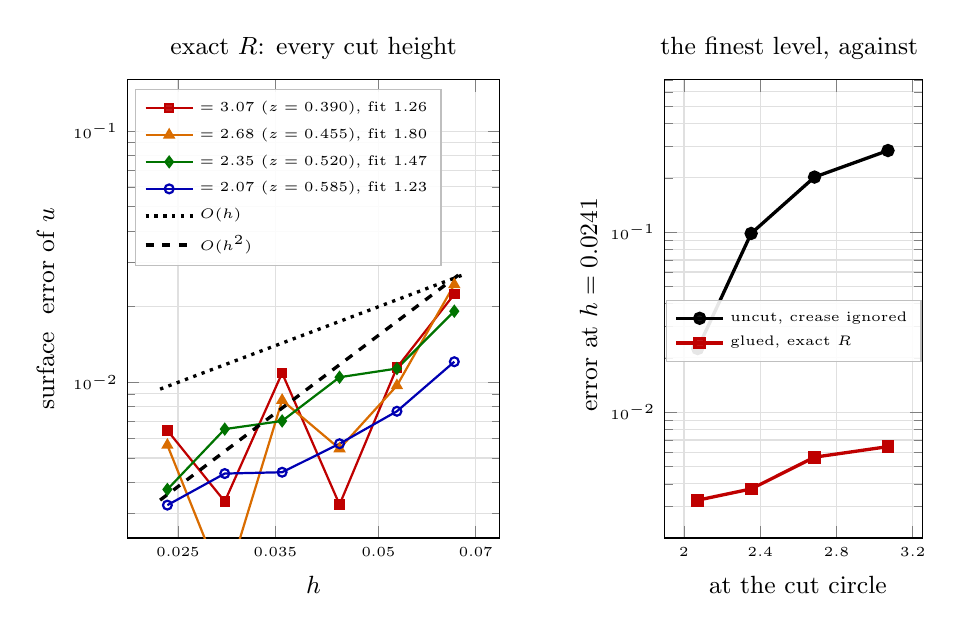
\begin{tikzpicture}

\begin{loglogaxis}[
  name=left,
  width=0.52\textwidth, height=7.4cm,
  xlabel={$h$}, ylabel={surface $\Linf$ error of $u$},
  title={\small exact $R$: every cut height},
  title style={yshift=-2pt},
  legend style={font=\tiny, at={(0.02,0.98)}, anchor=north west,
                draw=black!25, fill=white, fill opacity=0.9,
                text opacity=1, legend columns=1, row sep=0.5pt},
  legend cell align=left,
  xmin=0.021, xmax=0.076, ymin=2.4e-3, ymax=0.16,
  grid=both, grid style={black!12},
  tick label style={font=\tiny}, label style={font=\small},
  xtick={0.025,0.035,0.05,0.07},
  xticklabels={0.025,0.035,0.05,0.07},
]

\addplot[red!75!black, thick, mark=square*, mark size=1.5]
  coordinates {
    (0.065,2.244e-2) (0.053300,1.145e-2) (0.043706,3.261e-3)
    (0.035839,1.089e-2) (0.029388,3.356e-3) (0.024098,6.436e-3)};
\addlegendentry{$\dk=3.07$ ($z=0.390$), fit 1.26}

\addplot[orange!85!black, thick, mark=triangle*, mark size=1.8]
  coordinates {
    (0.065,2.451e-2) (0.053300,9.706e-3) (0.043706,5.444e-3)
    (0.035839,8.485e-3) (0.029388,1.516e-3) (0.024098,5.624e-3)};
\addlegendentry{$\dk=2.68$ ($z=0.455$), fit 1.80}

\addplot[green!45!black, thick, mark=diamond*, mark size=1.8]
  coordinates {
    (0.065,1.920e-2) (0.053300,1.135e-2) (0.043706,1.048e-2)
    (0.035839,7.020e-3) (0.029388,6.515e-3) (0.024098,3.747e-3)};
\addlegendentry{$\dk=2.35$ ($z=0.520$), fit 1.47}

\addplot[blue!70!black, thick, mark=o, mark size=1.6]
  coordinates {
    (0.065,1.208e-2) (0.053300,7.672e-3) (0.043706,5.697e-3)
    (0.035839,4.387e-3) (0.029388,4.334e-3) (0.024098,3.245e-3)};
\addlegendentry{$\dk=2.07$ ($z=0.585$), fit 1.23}

\addplot[black, dotted, very thick, domain=0.0235:0.067, samples=2]
  {2.6e-2*x/0.065};
\addlegendentry{$O(h)$}

\addplot[black, dashed, very thick, domain=0.0235:0.067, samples=2]
  {2.6e-2*(x/0.065)^2};
\addlegendentry{$O(h^2)$}

\end{loglogaxis}

\begin{semilogyaxis}[
  name=right, at={(left.east)}, anchor=west, xshift=2.1cm,
  width=0.40\textwidth, height=7.4cm,
  xlabel={$\dk$ at the cut circle},
  ylabel={$\Linf$ error at $h=0.0241$},
  ylabel style={yshift=-2pt},
  title={\small the finest level, against $\dk$},
  title style={yshift=-2pt},
  legend style={font=\tiny, at={(0.5,0.52)}, anchor=north,
                draw=black!25, fill=white, fill opacity=0.9,
                text opacity=1},
  legend cell align=left,
  xmin=1.9, xmax=3.25, ymin=2e-3, ymax=0.7,
  grid=both, grid style={black!12},
  tick label style={font=\tiny}, label style={font=\small},
  xtick={2.0,2.4,2.8,3.2},
]

\addplot[black, very thick, mark=*, mark size=1.8]
  coordinates {(2.0720,2.255e-2) (2.3525,9.824e-2)
               (2.6849,2.020e-1) (3.0703,2.836e-1)};
\addlegendentry{uncut, crease ignored}

\addplot[red!75!black, very thick, mark=square*, mark size=1.7]
  coordinates {(2.0720,3.245e-3) (2.3525,3.747e-3)
               (2.6849,5.624e-3) (3.0703,6.436e-3)};
\addlegendentry{glued, exact $R$}

\end{semilogyaxis}

\end{tikzpicture}
\caption{All four cut heights. Left: the surface $\Linf$ error of the
  glued solve with the exact rotation, against $h$. The uncut baseline is
  left out of this panel, because it is two orders of magnitude higher;
  it appears in Figure~\ref{fig:cut039} and in the right panel here. All
  four glued curves sit between the $O(h)$ and $O(h^2)$ guides, and all
  four zigzag. Right: the error at the finest level, against the
  curvature mismatch $\dk$. Both the baseline and the glued solve order
  monotonically by $\dk$, although the \emph{fitted slopes} do not ---
  see the text below.}
\label{fig:cutsummary}
\end{figure}


The four cut heights span crease angles from $34.9^\circ$ to
$81.8^\circ$, and with them a range of curvature mismatch.
Table~\ref{tab:fourcuts} collects them.

\begin{table}[htbp]
\centering
\caption{All four cuts of the flipped ellipsoid. $\dk$ falls as the cut
  moves from the equator towards the pole. Each entry is the fitted
  slope over six levels, with the error at the finest level
  ($h=0.0241$) beside it.}
\label{tab:fourcuts}
\footnotesize
\setlength{\tabcolsep}{4pt}
\begin{tabular}{@{}rrcrr rr rr rr rr@{}}
\toprule
 & & & &
 & \multicolumn{2}{c}{uncut, crease ignored}
 & \multicolumn{2}{c}{$d_k$}
 & \multicolumn{2}{c}{$d_{k2}$}
 & \multicolumn{2}{c}{exact $R$} \\
\cmidrule(lr){6-7}\cmidrule(lr){8-9}\cmidrule(lr){10-11}\cmidrule(lr){12-13}
$z$ & $\varphi_c$ & crease & $\kappa_m$ & $\dk$
 & rate & error & rate & error & rate & error & rate & error \\
\midrule
0.390 & 0.9273 & $81.8^\circ$ & 1.2986 & 3.0703
 & 0.10 & 2.84e-01 & 1.20 & 6.45e-03 & 2.31 & 6.41e-03 & 1.26 & 6.44e-03 \\
0.455 & 0.7954 & $67.1^\circ$ & 1.0970 & 2.6849
 & 0.59 & 2.02e-01 & 1.78 & 5.60e-03 & 2.20 & 5.80e-03 & 1.80 & 5.62e-03 \\
0.520 & 0.6435 & $52.0^\circ$ & 0.9220 & 2.3525
 & 0.33 & 9.82e-02 & 1.47 & 3.74e-03 & 1.89 & 3.70e-03 & 1.47 & 3.75e-03 \\
0.585 & 0.4510 & $34.9^\circ$ & 0.7738 & 2.0720
 & 1.00 & 2.25e-02 & 1.22 & 3.26e-03 & 1.22 & 3.28e-03 & 1.23 & 3.24e-03 \\
\bottomrule
\end{tabular}
\end{table}

\paragraph{The error level orders by $\dk$. The fitted rate does not.}
This is the main qualification on this test. At the finest level the
error of the glued solve falls monotonically as $\dk$ falls:
\begin{equation*}
  6.44,\quad 5.62,\quad 3.75,\quad 3.25 \;\;(\times 10^{-3})
  \qquad\text{for}\qquad
  \dk = 3.07,\; 2.68,\; 2.35,\; 2.07 .
\end{equation*}
The uncut baseline does the same, and far more strongly: from
$2.84\times10^{-1}$ down to $2.25\times10^{-2}$, a factor of 12.

The fitted slopes, by contrast, are $1.26$, $1.80$, $1.47$ and $1.23$.
They do not order by $\dk$, and they do not order by anything else
either. Six levels are not enough to separate a trend in the rate from
the grid-alignment scatter of Section~\ref{sec:scatter}. The defensible
statement from this study is therefore:

\begin{quote}
  Every cut converges at a fitted rate between $1.2$ and $1.8$. None
  reaches second order. The size of the error at a fixed grid spacing
  grows with $\dk$, as Equation~\eqref{eq:bound3} says it should ---
  through the constant in $C\,h\,D$, not through the exponent.
\end{quote}

That is how a bound behaves when its junction term is first order with a
$\dk$-dependent constant. Changing $\dk$ moves the curve up and down. It
would change the \emph{rate} only if $\dk$ reached zero. The unflipped
cut, where $\dk$ vanishes identically, is the test of that. It is the
\texttt{flipped = false} branch of the script, and it is not run here.

\paragraph{Where the error sits.} The script reports the distance of the
worst point from the cut circle, in units of $h$. At the two sharpest
cuts that distance is within one cell at nearly every level. At the
mildest cut, $z=0.585$, it is $11.5$, $14.1$ and $16.6$ cells at the
three coarsest levels, and it moves to the crease only at the three
finest. At a mild crease the junction is not the worst thing in the
solve until the grid is fine enough for the interior error to fall below
it.

\paragraph{The estimated rotations, across all cuts.} At every cut the
three variants agree at the finest level to within 1 per cent. The
fitted rates of the angle error are $2.13$, $2.30$, $2.36$ and $1.98$
for $d_k$, and $3.60$, $3.25$, $3.76$ and $2.93$ for $d_{k2}$. Both
estimators beat the nominal order of their underlying difference at
every cut, and neither difference reaches the solution.

